% Section 3.3:  Does the Strategy have a Context?  How is the ConcreteStrategy chosen?

\section{Software Patterns Present in SST}
The following patterns can be observed to have been already implemented in the project:
\begin{enumerate}
    \item Factory method pattern
    \item Singleton pattern
    \item Prototype pattern
          % \item Strategy pattern
\end{enumerate}
Other patterns are present in the project, such as C++ idioms (Include Guard Macro, enable\_if, etc.)

% Section 3.1:  Make sure to explain why you have both AF and FM patterns here.  Is one implementing the other?
% Explain whether or not the variadic form is consistent with the pattern.  Just from the function signature that you've shown I'm not sure that it is.
% In general be sure to explain all of the roles of the pattern and how they are filled by the implementation or not.  Roles include not just the classes, but the relationships and methods, too.
% Explain how the implementation deals with issues that were part of our discussion, for example, how is the client configured with a particular ConcreteCreator?

\subsection{Abstract Factory Pattern}
The abstract factory pattern is present in the \texttt{SST::Factory} class. In the repository, the class can be located at \texttt{factory.h}. The class is used to create several concrete products, including \texttt{Component} and \texttt{Module} objects.

The following figure lists the methods of the class following the typical steps dictated by the pattern.

% The following excerpt lists the methods of the class following the typical steps dictated by the pattern.

% \begin{lstlisting}[style=customC++,label=fm,caption=Factory Implementing the Abstract Factory Pattern]
% // src/sst/core/factory.h
% Component* CreateComponent(...);
% Module* CreateModule(...);
% Module* CreateModuleWithComponent(...);
% Partition::SSTPartitioner* CreatePartitioner(...);
% \end{lstlisting}

\begin{figure}[h]
    \caption{Factory Implementing the Abstract Factory Pattern}
    \centering
    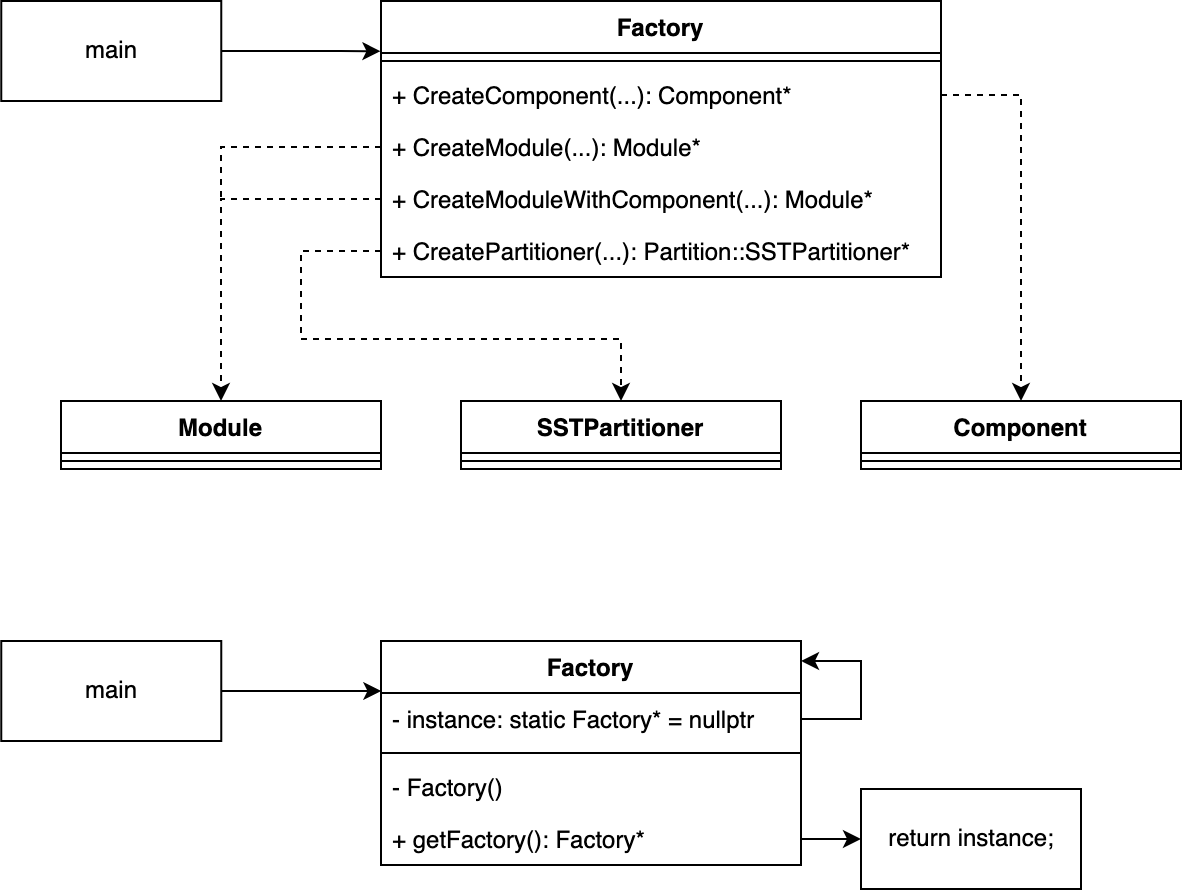
\includegraphics[width=0.8\textwidth]{af.png}
\end{figure}

% Section 3.2:  Is the Singleton implemented correctly?  Does it have any special features that help it deal with being instantiated in a multi-threaded environment, like locks, DCL or being instantiated at a particular place in the program?  Is it ever destroyed?

\subsection{Singleton Pattern}
The singleton pattern is present in the \texttt{SST::Factory} class. In the repository, the class can be located at \texttt{factory.h}. The class is used to instantiate other concrete simulation classes. SST requires simulation objects to be synchronized throughout the kernel, especially since they can be running on a distributed system where race conditions can become major issues. The software forces these simulation objects to be Singletons.

\begin{figure}[h]
    \caption{Factory Implementing the Singleton Pattern}
    \centering
    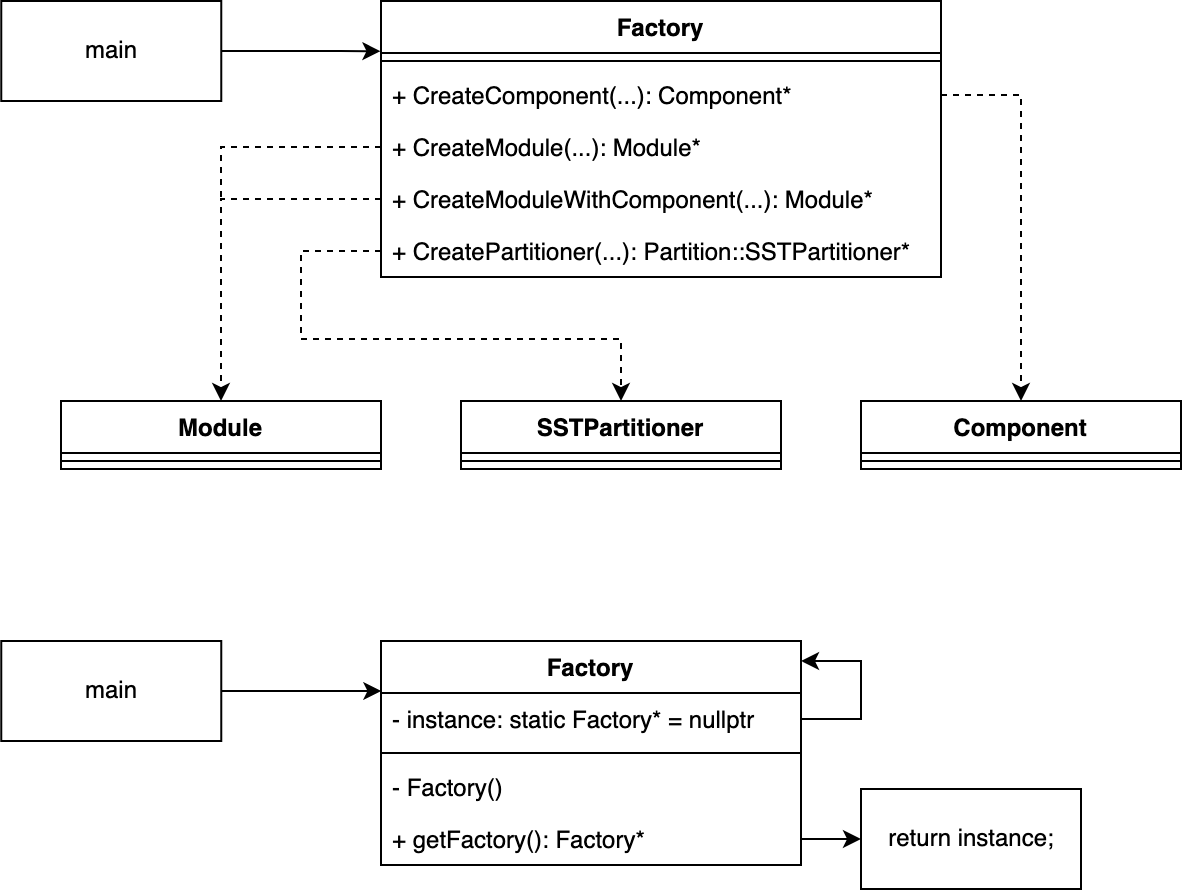
\includegraphics[width=0.8\textwidth]{singleton.png}
\end{figure}
\newpage

The following listing consolidates all instances of the class following the typical steps dictated by the pattern.

\begin{lstlisting}[style=customC++,label=singleton,caption=Factory Implementing the Singleton Pattern \\ File: src/sst/core/factory.h and src/sst/core/factory.cc]
class Factory {
    Factory(const std::string& searchPaths);
    ~Factory();
    static Factory* instance;
}

Factory* Factory::instance = nullptr;

Factory::Factory(...) {
    if (instance) {
        out.fatal(CALL_INFO, 1, "Already initialized a factory.\n");
    }
    instance = this;
}
\end{lstlisting}

Although SST is primarily intended for multi-threaded applications, the Singleton class does not utilize any locks to account for the potential issues imposed by concurrency. Locks do exist in abundance throughout the project and within the class itself, but not when checking for instances of itself in other threads. The \texttt{Factory} class is responsible for creating SST Components, SubComponents, Modules, etc. as models for the simulation. It appears that the Singleton is instantiated by \texttt{mpirun} as a single thread which spawns the other processes after it completes analysis of the configuration options. The intent of the pattern is still preserved, although with the aforementioned assumptions that the executable instantiates it with a single thread.

The safety of the Singleton can be improved with the usage of mutexes to implement a double-checked locking \cite{dcl}, which is cited as an efficient method for implementing lazy initialization in a multi-threaded environment.

% \subsection{Strategy pattern}
% The Strategy pattern is present in the \texttt{SST::Core::Serialization::serializer} class. The class is implemented throughout multiple files in \texttt{serialization}, where it is overloaded in the files with various parameter types, with all the various versions of the class simply overloading the function call operator (\texttt{operator()}).

\newpage
\subsection{Prototype Pattern}
The Prototype pattern is present in the project, although in a very limited manner. Select \texttt{SST::Core::Interfaces} classes implement a \texttt{clone} method to provide the ability to copy instances of themselves. The \texttt{StringEvent} class provides a shallow copy of itself to instantiate its ConcretePrototype, while \texttt{SimpleNetwork::Request} performs a deep copy.

\begin{figure}[h]
    \caption{Factory Implementing the Prototype Pattern}
    \centering
    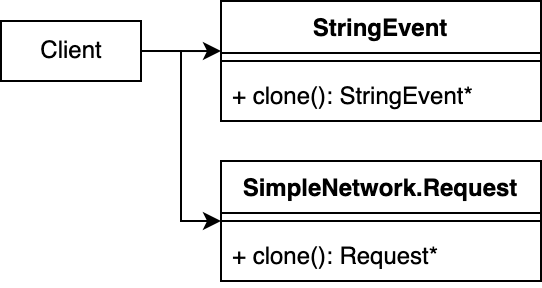
\includegraphics[width=0.8\textwidth]{proto.png}
\end{figure}

The following listings demonstrate the instances of the project following the typical steps dictated by the pattern:

\begin{lstlisting}[style=customC++,label=prototype1,caption=StringEvent Implementing the Prototype Pattern \\ File: src/sst/core/interfaces/stringEvent.h]
class StringEvent : public SST::Event, ... {
    virtual Event* clone() override {
        return new StringEvent(*this);
    }
}
\end{lstlisting}

\begin{lstlisting}[style=customC++,label=prototype2,caption=SimpleNetwork::Request Implementing the Prototype Pattern \\ File: src/sst/core/interfaces/simpleNetwork.h]
class SimpleNetwork : public SubComponent {
    class Request : public ... {
        inline Request* clone() {
            Request* req = new Request(*this);
            // Copy constructor only makes a shallow copy, need to
            // clone the event.
            if (payload != nullptr) {
                req->payload = payload->clone();
            }
            return req;
        }
    }
}
\end{lstlisting}
